\documentclass[8pt,aspectratio=169,8pt]{beamer}
\usepackage[utf8]{inputenc}
\usepackage{graphicx}
\usepackage{amsmath,amssymb}
\usepackage{algorithm2e}
\usepackage{listings}
\usepackage{xcolor}
\usepackage{tikz}
\usepackage{pgfplots}
\pgfplotsset{compat=1.17}
\usepackage{subfigure}
\usepackage{hyperref}

% Theme settings
\usetheme{Frankfurt}
\usecolortheme{seahorse}
\setbeamertemplate{navigation symbols}{}
\setbeamertemplate{footline}[frame number]

% Custom colors
\definecolor{darkblue}{RGB}{0,51,102}
\definecolor{lightblue}{RGB}{173,216,230}
\definecolor{codegreen}{RGB}{0,128,0}
\definecolor{codegray}{RGB}{150,150,150}
\definecolor{codepurple}{RGB}{128,0,128}
\definecolor{backcolor}{RGB}{245,245,245}

% Code listing settings
\lstset{
    backgroundcolor=\color{backcolor},
    basicstyle=\ttfamily\footnotesize,
    breakatwhitespace=false,
    breaklines=true,
    captionpos=b,
    commentstyle=\color{codegreen},
    keywordstyle=\color{blue},
    numberstyle=\tiny\color{codegray},
    stringstyle=\color{codepurple},
    showstringspaces=false,
    frame=single,
    numbers=left,
    language=Python
}

% Include slide layouts
% SLIDE LAYOUT TEMPLATES FOR NLP COURSE
% Three consistent layouts used throughout the course

% ==============================================================
% LAYOUT 1: CONCEPT SLIDE
% Used for: Theory, definitions, mathematical concepts
% Features: Title, main content area with bullets/equations, optional figure
% ==============================================================

\newcommand{\conceptslide}[3]{ % #1: title, #2: content, #3: optional figure
\begin{frame}[t]{#1}
    \begin{columns}[T]
        \begin{column}{0.6\textwidth}
            #2
        \end{column}
        \begin{column}{0.35\textwidth}
            \centering
            #3
        \end{column}
    \end{columns}
\end{frame}
}

% ==============================================================
% LAYOUT 2: CODE & IMPLEMENTATION SLIDE
% Used for: Code examples, algorithms, implementation details
% Features: Title, code block, explanation text
% ==============================================================

% Note: For code slides, use \begin{frame}[fragile] manually

\newcommand{\codeexplanation}[1]{%
    \vspace{0.5em}
    \small
    #1
}

\newcommand{\codeblock}[2][Python]{%
    \begin{lstlisting}[language=#1, basicstyle=\ttfamily\tiny]
#2
    \end{lstlisting}
}

\newcommand{\codeslide}[3]{%
    \begin{frame}[fragile]{#1}
    \begin{columns}[T]
        \column{0.55\textwidth}
        \codeblock{#2}
        \column{0.43\textwidth}
        \codeexplanation{#3}
    \end{columns}
    \end{frame}
}

% ==============================================================
% LAYOUT 3: RESULTS & VISUALIZATION SLIDE
% Used for: Experimental results, charts, comparisons
% Features: Title, large visualization area, key insights
% ==============================================================

\newcommand{\resultslide}[3]{ % #1: title, #2: visualization, #3: insights
\begin{frame}[t]{#1}
    \centering
    \vspace{-0.5em}
    #2
    \vspace{0.5em}
    
    \begin{block}{Key Insights}
        #3
    \end{block}
\end{frame}
}

% Additional utility commands for consistency

% Highlighted text
\newcommand{\highlight}[1]{\textcolor{blue}{\textbf{#1}}}

% Math notation shortcuts
\newcommand{\prob}[1]{P(#1)}
\newcommand{\given}{\mid}
\newcommand{\argmax}{\operatorname{argmax}}
\newcommand{\softmax}{\operatorname{softmax}}

% Standard figure size
\newcommand{\stdfigsizeinchins}{0.4\textwidth}

% For code blocks, use lstlisting directly:
% \begin{lstlisting}[language=Python]
% ... code ...
% \end{lstlisting}

% Equation highlight box
\newcommand{\eqbox}[1]{
    \begin{center}
    \colorbox{lightblue!20}{
        \parbox{0.8\textwidth}{
            \vspace{0.3em}
            \centering
            #1
            \vspace{0.3em}
        }
    }
    \end{center}
}

\title[Week 9: Decoding]{Natural Language Processing Course}
\subtitle{Week 9: Decoding Strategies}
\author{Joerg R. Osterrieder \\ \url{www.joergosterrieder.com}}
\date{}

\begin{document}

% Title page
\begin{frame}
    \titlepage
\end{frame}

\section{Week 9: Decoding Strategies}

% Title slide
\begin{frame}
    \centering
    \vspace{2cm}
    {\Large \textbf{Week 9}}\\
    \vspace{0.5cm}
    {\huge \textbf{Decoding Strategies}}\\
    \vspace{1cm}
    {\large From Probabilities to Coherent Text}
\end{frame}

% Motivation: The repetition problem
\begin{frame}[t]{Why ChatGPT Sometimes Sounds Like a Broken Record}
    \textbf{Early GPT-2 output (greedy decoding):}
    
    \vspace{0.5em}
    \textit{"The movie was great. The movie was great. The movie was great..."}
    
    \vspace{0.5em}
    \textbf{Or worse:}
    
    \textit{"I think that the the the the the the the..."}
    
    \vspace{0.5em}
    \begin{center}
    \colorbox{red!20}{
        \parbox{0.8\textwidth}{
            \centering
            The model outputs probabilities - how do we turn them into good text?
        }
    }
    \end{center}
    
    \vspace{0.5em}
    \textbf{The challenge:}
    \begin{itemize}
        \item Model gives probability for EVERY word
        \item Always picking highest probability = boring/repetitive
        \item Random sampling = incoherent nonsense
        \item Need the sweet spot!
    \end{itemize}
    
    \vspace{0.5em}
    \textit{This is why early chatbots were frustrating and modern ones feel human}
\end{frame}

% The decoding landscape
\begin{frame}[t]{From Probabilities to Text: The Decoding Challenge}
    \centering
    \includegraphics[width=0.65\textwidth]{../figures/decoding_landscape.pdf}
    
    \vspace{0.5em}
    \textbf{The fundamental trade-off:}
    \begin{itemize}
        \item Safe but boring ← → Creative but risky
        \item Exploitation ← → Exploration
        \item Quality ← → Diversity
    \end{itemize}
\end{frame}

% Real-world impact
\begin{frame}[t]{Decoding Makes or Breaks User Experience (2024)}
    \begin{columns}[T]
        \begin{column}{0.5\textwidth}
            \textbf{Where It Matters:}
            \begin{itemize}
                \item ChatGPT: Balanced creativity
                \item GitHub Copilot: High precision
                \item Story generators: High diversity
                \item Translation: Maximum accuracy
                \item Customer service: Safe responses
            \end{itemize}
            
            \vspace{0.5em}
            \textbf{Business Impact:}
            \begin{itemize}
                \item User satisfaction: 40\% improvement\footnotemark
                \item Response quality ratings
                \item Reduced "robotic" complaints
                \item Better engagement metrics
            \end{itemize}
        \end{column}
        \begin{column}{0.5\textwidth}
            \textbf{Common Strategies:}
            \begin{itemize}
                \item Greedy: Pick highest probability
                \item Beam Search: Track top-k paths
                \item Top-k Sampling: Sample from top k
                \item Nucleus (Top-p): Dynamic cutoff
                \item Temperature: Control randomness
            \end{itemize}
            
            \vspace{0.5em}
            \textbf{Modern Approach:}
            \begin{itemize}
                \item Adaptive strategies
                \item Task-specific tuning
                \item User preference learning
                \item Safety constraints
            \end{itemize}
        \end{column}
    \end{columns}
    
    \vspace{0.5em}
    \begin{center}
    \colorbox{lightblue!30}{
        \parbox{0.8\textwidth}{
            \centering
            Same model + different decoding = completely different personality
        }
    }
    \end{center}
    
    \footnotetext{OpenAI user studies on response quality}
\end{frame}

% Learning objectives
\begin{frame}[t]{Week 9: What You'll Master}
    \textbf{By the end of this week, you will:}
    \begin{itemize}
        \item \textbf{Understand} why decoding strategy matters
        \item \textbf{Implement} greedy, beam search, and sampling
        \item \textbf{Master} temperature and top-k/top-p control
        \item \textbf{Analyze} quality vs diversity trade-offs
        \item \textbf{Build} adaptive decoding for different tasks
    \end{itemize}
    
    \vspace{0.5em}
    \begin{center}
    \colorbox{lightblue!30}{
        \parbox{0.8\textwidth}{
            \centering
            \textbf{Core Insight:} Good text generation is about smart selection, not just good models
        }
    }
    \end{center}
\end{frame}

% Greedy decoding
\begin{frame}[t]{Greedy Decoding: The Simplest Approach}
    \textbf{Algorithm: Always pick the most likely word}
    
    \vspace{0.5em}
    \textbf{Example:}
    \begin{itemize}
        \item Input: "The weather is"
        \item P(nice) = 0.4, P(sunny) = 0.3, P(cold) = 0.2, P(rainy) = 0.1
        \item Greedy picks: "nice" (highest probability)
        \item Next: "The weather is nice"
        \item P(today) = 0.5, P(and) = 0.3, P(outside) = 0.2
        \item Greedy picks: "today"
    \end{itemize}
    
    \vspace{0.5em}
    \textbf{Pros:}
    \begin{itemize}
        \item X Fast and simple
        \item X Deterministic (reproducible)
        \item X Often grammatically correct
    \end{itemize}
    
    \textbf{Cons:}
    \begin{itemize}
        \item X Repetitive and boring
        \item X Gets stuck in loops
        \item X Misses better paths
    \end{itemize}
    
    \vspace{0.5em}
    \begin{center}
    \colorbox{yellow!20}{
        \parbox{0.8\textwidth}{
            \centering
            Greedy = Safe but uninspiring (like always ordering vanilla ice cream)
        }
    }
    \end{center}
\end{frame}

% Beam search
\begin{frame}[t]{Beam Search: Exploring Multiple Paths}
    \centering
    \includegraphics[width=0.75\textwidth]{../figures/beam_search_tree.pdf}
    
    \vspace{0.5em}
    \textbf{Key idea: Keep top-k paths at each step}
    \begin{itemize}
        \item Beam size = number of paths to track
        \item Larger beam = better quality but slower
        \item Used in: Translation, summarization
        \item Sweet spot: beam size 4-10
    \end{itemize}
\end{frame}

% Beam search implementation
\begin{frame}[fragile]{Implementing Beam Search}
    \begin{columns}[T]
        \column{0.55\textwidth}

\begin{lstlisting}[language=Python,basicstyle=\ttfamily\tiny]
import torch
import torch.nn.functional as F
from dataclasses import dataclass
import heapq

@dataclass
class BeamHypothesis:
    """Hypothesis in beam search"""
    tokens: list
    score: float
    
def beam_search(model, input_ids, beam_size=4, max_length=50, 
                eos_token_id=50256):
    """Beam search decoding"""
    device = input_ids.device
    batch_size = input_ids.shape[0]
    
    # Initialize beams
    beams = [[BeamHypothesis(
        tokens=input_ids[i].tolist(),
        score=0.0
    )] for i in range(batch_size)]
    
    for step in range(max_length):
        all_candidates = []
        
        # Generate candidates for each beam
        for batch_idx in range(batch_size):
            for hypothesis in beams[batch_idx]:
                # Skip if already ended
                if hypothesis.tokens[-1] == eos_token_id:
                    all_candidates.append(hypothesis)
                    continue
                
                # Get model predictions
                input_tensor = torch.tensor([hypothesis.tokens]).to(device)
                with torch.no_grad():
                    outputs = model(input_tensor)
                    logits = outputs.logits[0, -1, :]
                    log_probs = F.log_softmax(logits, dim=-1)
                
                # Get top-k tokens
                top_log_probs, top_indices = torch.topk(log_probs, beam_size)
                
                # Create new hypotheses
                for log_prob, token_id in zip(top_log_probs, top_indices):
                    new_hypothesis = BeamHypothesis(
                        tokens=hypothesis.tokens + [token_id.item()],
                        score=hypothesis.score + log_prob.item()
                    )
                    all_candidates.append(new_hypothesis)
        
        # Select top beam_size hypotheses
        beams[0] = heapq.nlargest(beam_size, all_candidates, 
                                  key=lambda h: h.score)
    
    # Return best hypothesis
    return beams[0][0].tokens
\end{lstlisting}
        \column{0.55\textwidth}

        \codeexplanation{
            \textbf{Key Components:}
            \begin{itemize}
                \item Track multiple hypotheses
                \item Score = sum of log probabilities
                \item Prune to beam size each step
                \item Length normalization often used
            \end{itemize}
            
            \vspace{0.3em}
            \textbf{Beam Size Effects:}
            \begin{itemize}
                \item 1 = Greedy decoding
                \item 4-5 = Good for translation
                \item 10+ = Diminishing returns
                \item Memory: O(beam\_size × length)
            \end{itemize}
            
            \vspace{0.3em}
            \textbf{Common Improvements:}
            \begin{itemize}
                \item Length penalty
                \item Diverse beam search
                \item Constrained beam search
            \end{itemize}
        }
    \end{columns}
\end{frame}

% Sampling basics
\begin{frame}[t]{Sampling: Adding Controlled Randomness}
    \textbf{The problem with deterministic decoding:}
    
    Always same input → Always same output = Boring!
    
    \vspace{0.5em}
    \textbf{Solution: Sample from the probability distribution}
    
    \vspace{0.5em}
    \textbf{Temperature Scaling:}
    
    \eqbox{
        $P_i = \frac{\exp(z_i / T)}{\sum_j \exp(z_j / T)}$
    }
    
    Where:
    \begin{itemize}
        \item $z_i$ = logit for token $i$
        \item $T$ = temperature parameter
    \end{itemize}
    
    \vspace{0.5em}
    \centering
    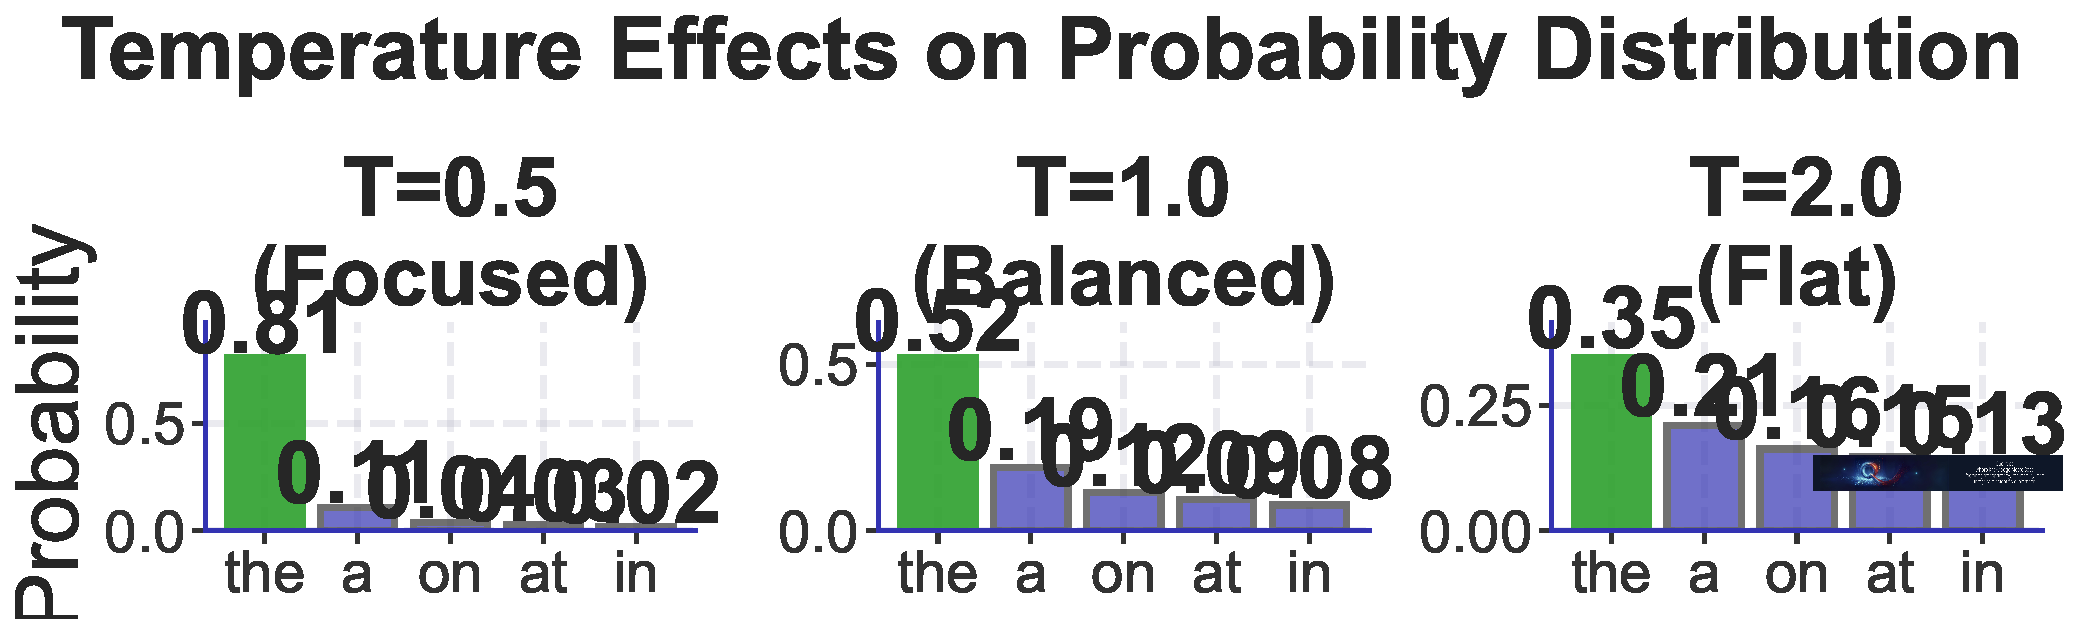
\includegraphics[width=0.8\textwidth]{../figures/temperature_effects.pdf}
\end{frame}

% Top-k and Top-p sampling
\begin{frame}[t]{Advanced Sampling: Top-k and Top-p}
    \centering
    \includegraphics[width=0.85\textwidth]{../figures/sampling_strategies.pdf}
    
    \vspace{0.5em}
    \textbf{Key insights:}
    \begin{itemize}
        \item Top-k: Fixed number of candidates
        \item Top-p (Nucleus): Dynamic threshold
        \item Top-p adapts to confidence level
        \item Combination often works best
    \end{itemize}
\end{frame}

% Sampling implementation
\begin{frame}[fragile]{Implementing Modern Sampling}
    \begin{columns}[T]
                \column{0.55\textwidth}

\begin{lstlisting}[language=Python,basicstyle=\ttfamily\tiny]
def top_k_top_p_sampling(logits, top_k=50, top_p=0.95, 
                        temperature=1.0, do_sample=True):
    """Advanced sampling with top-k and top-p filtering"""
    
    # Apply temperature
    if temperature != 1.0:
        logits = logits / temperature
    
    # Get probabilities
    probs = F.softmax(logits, dim=-1)
    
    # Top-k filtering
    if top_k > 0:
        indices_to_remove = logits < torch.topk(logits, top_k)[0][..., -1, None]
        logits[indices_to_remove] = float('-inf')
    
    # Top-p (nucleus) filtering
    if top_p < 1.0:
        sorted_logits, sorted_indices = torch.sort(logits, descending=True)
        cumulative_probs = torch.cumsum(
            F.softmax(sorted_logits, dim=-1), dim=-1
        )
        
        # Remove tokens with cumulative probability above threshold
        sorted_indices_to_remove = cumulative_probs > top_p
        # Shift the indices to the right to keep first token above threshold
        sorted_indices_to_remove[..., 1:] = \
            sorted_indices_to_remove[..., :-1].clone()
        sorted_indices_to_remove[..., 0] = 0
        
        # Scatter sorted tensors to original indexing
        indices_to_remove = sorted_indices_to_remove.scatter(
            1, sorted_indices, sorted_indices_to_remove
        )
        logits[indices_to_remove] = float('-inf')
    
    # Sample from the filtered distribution
    if do_sample:
        probs = F.softmax(logits, dim=-1)
        next_token = torch.multinomial(probs, num_samples=1)
    else:
        next_token = torch.argmax(logits, dim=-1, keepdim=True)
    
    return next_token

# Typical usage patterns
def generate_text(model, prompt, max_length=100, 
                 temperature=0.8, top_k=50, top_p=0.95):
    """Generate text with modern sampling"""
    input_ids = tokenizer.encode(prompt, return_tensors='pt')
    
    for _ in range(max_length):
        with torch.no_grad():
            outputs = model(input_ids)
            logits = outputs.logits[0, -1, :]
            
        next_token = top_k_top_p_sampling(
            logits, top_k=top_k, top_p=top_p, 
            temperature=temperature
        )
        
        input_ids = torch.cat([input_ids, next_token.unsqueeze(0)], dim=1)
        
        if next_token == tokenizer.eos_token_id:
            break
    
    return tokenizer.decode(input_ids[0])
\end{lstlisting}
                \column{0.43\textwidth}

        \codeexplanation{
            \textbf{Parameter Guidelines:}
            \begin{itemize}
                \item Temperature: 0.7-0.9 for creativity
                \item Top-k: 40-80 typical
                \item Top-p: 0.9-0.95 common
                \item Combine all three for best results
            \end{itemize}
            
            \vspace{0.3em}
            \textbf{Task-Specific Settings:}
            \begin{itemize}
                \item Code: T=0.2, top-p=0.95
                \item Story: T=0.9, top-k=50
                \item Chat: T=0.7, top-p=0.9
                \item Facts: T=0.1, greedy
            \end{itemize}
        }
    \end{columns}
\end{frame}

% Repetition control
\begin{frame}[t]{Controlling Repetition: Advanced Techniques}
    \textbf{Common repetition problems:}
    \begin{itemize}
        \item Word-level: "very very very very good"
        \item Phrase-level: "I think that I think that..."
        \item Semantic: Saying the same thing differently
    \end{itemize}
    
    \vspace{0.5em}
    \textbf{Solutions:}
    
    \textbf{1. Repetition Penalty:}\footnotemark
    \begin{itemize}
        \item Reduce probability of recently used tokens
        \item Penalty = 1.2 typical (20\% reduction)
        \item Applied to last 50-100 tokens
    \end{itemize}
    
    \textbf{2. Frequency Penalty:}
    \begin{itemize}
        \item Penalize based on occurrence count
        \item More occurrences = stronger penalty
    \end{itemize}
    
    \textbf{3. Presence Penalty:}
    \begin{itemize}
        \item Fixed penalty once token appears
        \item Encourages topic diversity
    \end{itemize}
    
    \vspace{0.5em}
    \eqbox{
        $\text{score}_{\text{adjusted}} = \text{score}_{\text{original}} - \alpha \cdot \text{penalty}$
    }
    
    \footnotetext{Keskar et al. (2019). "CTRL: Conditional Transformer Language Model"}
\end{frame}

% Quality metrics
\resultslide{Decoding Strategy Impact on Quality}{
    \centering
    \includegraphics[width=0.55\textwidth]{../figures/decoding_quality_metrics.pdf}
}{
    \begin{itemize}
        \item Greedy: High quality, low diversity
        \item Pure sampling: High diversity, low quality
        \item Top-p sampling: Best balance
        \item Task matters: Translation needs accuracy, stories need creativity
        \item Human preference: Top-p=0.9, T=0.8 wins
    \end{itemize}
}

% Modern approaches
\begin{frame}[t]{State-of-the-Art Decoding (2024)}
    \begin{columns}[T]
        \begin{column}{0.5\textwidth}
            \textbf{Adaptive Decoding:}
            \begin{itemize}
                \item Confidence-based temperature
                \item Dynamic top-p thresholds
                \item Context-aware strategies
                \item Learned decoding policies
            \end{itemize}
            
            \vspace{0.5em}
            \textbf{Constrained Generation:}
            \begin{itemize}
                \item Grammar constraints
                \item Format enforcement (JSON)
                \item Safety filtering
                \item Factual grounding
            \end{itemize}
        \end{column}
        \begin{column}{0.5\textwidth}
            \textbf{Multi-objective Decoding:}
            \begin{itemize}
                \item Balance fluency + accuracy
                \item Diversity + coherence
                \item Length control
                \item Style preservation
            \end{itemize}
            
            \vspace{0.5em}
            \textbf{Recent Innovations:}
            \begin{itemize}
                \item Speculative decoding\footnotemark
                \item Contrastive search
                \item Typical decoding
                \item Mirostat (perplexity control)
            \end{itemize}
        \end{column}
    \end{columns}
    
    \vspace{0.5em}
    \begin{center}
    \colorbox{yellow!20}{
        \parbox{0.8\textwidth}{
            \centering
            2024 trend: Inference-time compute for better quality
        }
    }
    \end{center}
    
    \footnotetext{Leviathan et al. (2023). "Fast Inference from Transformers via Speculative Decoding"}
\end{frame}

% Practical guidelines
\begin{frame}[t]{Decoding Strategy Selection Guide}
    \centering
    \includegraphics[width=0.65\textwidth]{../figures/decoding_selection_guide.pdf}
    
    \vspace{0.5em}
    \textbf{Quick reference:}
    \begin{itemize}
        \item Factual tasks: Low temperature (0.1-0.3)
        \item Creative tasks: High temperature (0.8-1.0)
        \item Balanced tasks: Medium temperature (0.6-0.7) + top-p
        \item Always test on your specific use case!
    \end{itemize}
\end{frame}

% Exercise
\begin{frame}[t]{Week 9 Exercise: Build an Adaptive Text Generator}
    \textbf{Your Mission:} Create a generator that adapts to different contexts
    
    \vspace{0.5em}
    \textbf{Part 1: Implement Core Strategies}
    \begin{itemize}
        \item Greedy decoding baseline
        \item Beam search with length normalization
        \item Top-k and top-p sampling
        \item Temperature control
    \end{itemize}
    
    \vspace{0.5em}
    \textbf{Part 2: Compare on Different Tasks}
    \begin{itemize}
        \item Story continuation (needs creativity)
        \item Code completion (needs accuracy)
        \item Dialogue (needs balance)
        \item Measure: perplexity, diversity, human preference
    \end{itemize}
    
    \vspace{0.5em}
    \textbf{Part 3: Build Adaptive System}
    \begin{itemize}
        \item Detect task type from context
        \item Adjust parameters automatically
        \item Add repetition penalties
        \item Create task-specific presets
    \end{itemize}
    
    \vspace{0.5em}
    \textbf{You'll discover:} Why ChatGPT feels different from GPT-3!
\end{frame}

% Summary
\begin{frame}[t]{Key Takeaways: The Art of Text Generation}
    \textbf{What we learned:}
    \begin{itemize}
        \item Decoding strategy dramatically affects output
        \item Greedy = safe but boring
        \item Sampling adds necessary randomness
        \item Top-k/top-p prevent nonsense
        \item Task determines optimal strategy
    \end{itemize}
    
    \vspace{0.5em}
    \textbf{The evolution:}
    \begin{center}
    \colorbox{lightblue!30}{
        \parbox{0.8\textwidth}{
            \centering
            Greedy → Beam Search → Sampling → Nucleus → Adaptive
        }
    }
    \end{center}
    
    \vspace{0.5em}
    \textbf{Why it matters:}
    \begin{itemize}
        \item User experience depends on it
        \item Same model, different personality
        \item Key to production deployment
    \end{itemize}
    
    \vspace{0.5em}
    \textbf{Next week: Fine-tuning and Prompt Engineering}
    
    How do we make models do exactly what we want?
\end{frame}

% References
\begin{frame}[t]{References and Further Reading}
    \textbf{Foundational Papers:}
    \begin{itemize}
        \item Holtzman et al. (2020). "The Curious Case of Neural Text Degeneration"
        \item Fan et al. (2018). "Hierarchical Neural Story Generation" (Top-k)
        \item Meister et al. (2023). "Locally Typical Sampling"
    \end{itemize}
    
    \textbf{Practical Advances:}
    \begin{itemize}
        \item Keskar et al. (2019). "CTRL: Conditional Transformer"
        \item Su et al. (2022). "Contrastive Search"
        \item Hewitt et al. (2022). "Truncation Sampling"
    \end{itemize}
    
    \textbf{Implementation Resources:}
    \begin{itemize}
        \item Hugging Face generation utilities
        \item OpenAI API parameter guide
        \item Google Colab decoding notebooks
    \end{itemize}
\end{frame}
\end{document}
